%%%%%%%%%%%%%%%%%%%%%%%%%%%%%%%%%%%%%%%%%
% Beamer Presentation
% LaTeX Template
% Version 1.0 (10/11/12)
%
% This template has been downloaded from:
% http://www.LaTeXTemplates.com
%
% License:
% CC BY-NC-SA 3.0 (http://creativecommons.org/licenses/by-nc-sa/3.0/)
%
%%%%%%%%%%%%%%%%%%%%%%%%%%%%%%%%%%%%%%%%%

%----------------------------------------------------------------------------------------
%	PACKAGES AND THEMES
%----------------------------------------------------------------------------------------

\documentclass{beamer}
\usepackage{mathtools}
\usepackage{bm}
\usepackage{siunitx}
\usepackage{dsfont}
\usepackage{xspace}
\usepackage{longtable}
\usepackage{xifthen}

\input{math_commands}

%NB With beamer, the packages enumerate and paralist used for setting listing counters are not usable :(

\mode<presentation> {

% The Beamer class comes with a number of default slide themes
% which change the colors and layouts of slides. Below this is a list
% of all the themes, uncomment each in turn to see what they look like.

%\usetheme{default}
%\usetheme{AnnArbor}
%\usetheme{Antibes}
%\usetheme{Bergen}
%\usetheme{Berkeley}
%\usetheme{Berlin}
%\usetheme{Boadilla}
%\usetheme{CambridgeUS}
%\usetheme{Copenhagen}
%\usetheme{Darmstadt}
%\usetheme{Dresden}
%\usetheme{Frankfurt}
%\usetheme{Goettingen}
%\usetheme{Hannover}
%\usetheme{Ilmenau}
%\usetheme{JuanLesPins}
%\usetheme{Luebeck}
\usetheme{Madrid}
%\usetheme{Malmoe}
%\usetheme{Marburg}
%\usetheme{Montpellier}
%\usetheme{PaloAlto}
%\usetheme{Pittsburgh}
%\usetheme{Rochester}
%\usetheme{Singapore}
%\usetheme{Szeged}
%\usetheme{Warsaw}

% As well as themes, the Beamer class has a number of color themes
% for any slide theme. Uncomment each of these in turn to see how it
% changes the colors of your current slide theme.

%\usecolortheme{albatross}
%\usecolortheme{beaver} % among the best
%\usecolortheme{beetle}
\usecolortheme{crane} % among the best
%\usecolortheme{dolphin}
%\usecolortheme{dove}
%\usecolortheme{fly}
%\usecolortheme{lily}
%\usecolortheme{orchid}
%\usecolortheme{rose}
%\usecolortheme{seagull}
%\usecolortheme{seahorse}
%\usecolortheme{whale}
%\usecolortheme{wolverine}

%\setbeamertemplate{footline} % To remove the footer line in all slides uncomment this line
%\setbeamertemplate{footline}[page number] % To replace the footer line in all slides with a simple slide count uncomment this line

%\setbeamertemplate{navigation symbols}{} % To remove the navigation symbols from the bottom of all slides uncomment this line
}


\title{Interview Presentation: Random Planted Forests (RPFs)}
\author{Coco Bögel}
\date{\today}

\renewcommand*\contentsname{Summary}

\pdfinfo{%
  /Title    ()
  /Author   ()
  /Creator  ()
  /Producer ()
  /Subject  ()
  /Keywords ()
}



%BEACHTE: \label-Befehle müssen zu Beginn einer Gleichung, Satz etc. stehen, nicht anschließend, damit Nummerierung funktioniert


\nocite{RL, Slides, AtariDRL, DoubleQ, AlignmentProblem, Dayan, LaTeXSymbol, MLehn}


%----------------------------------------------------------------------------------------
%	TITLE PAGE
%----------------------------------------------------------------------------------------

\AtBeginSection[]
{
  \begin{frame}
    \frametitle{Outline}
    \tableofcontents[currentsection]
  \end{frame}
}

% \title{24-02-23_BMS_Stud_Conf_Talk}
% \author{Coco Bögel}
% \date{February 2024}

\title[Random Planted Forests (RPFs)]{Random Planted Forest: A Directly Interpretable Tree Ensemble (2023)} % The short title appears at the bottom of every slide, the full title is only on the title page

\author{Coco Bögel} % Your name
\institute[] % Your institution as it will appear on the bottom of every slide, may be shorthand to save space
{
\begin{large}
% \textit{}
Research paper by Munir Hiabu, \\ Enno Mammen and Joseph T. Meyer
\end{large}
\\ % Your institution for the title page
\medskip
\begin{small}
\textit{Talk at LMU Munich, Institute of Statistics} \\ % Your email address
\end{small}
\medskip
% \begin{normalsize}
% Application interview by Coco Bögel
% \end{normalsize}
}
\date{15th October 2024} % Date, can be changed to a custom date



\begin{document}

\begin{frame}
\titlepage % Print the title page as the first slide
\end{frame}

% \include{dummy_frame}



\begin{frame}
\frametitle{Outline} % Table of contents slide, comment this block out to remove it
\tableofcontents % Throughout your presentation, if you choose to use \section{} and \subsection{} commands, these will automatically be printed on this slide as an overview of your presentation
\end{frame}



%----------------------------------------------------------------------------------------
%	PRESENTATION SLIDES
%----------------------------------------------------------------------------------------



\section{Underlying ideas and general algorithm}



\subsection{Interaction order}

\begin{frame}{Interaction order and Interpretability}

    Interpretability by restricting to low \textit{interaction order} r

    \begin{figure}[h]
        \vspace{-10pt} % Note that this is only to ensure a normal, not to big margin around the figure
        %\centering
        \includegraphics[width=1.1\linewidth]{img/Bildschirmfoto_20241015_005914_BI_r_condition_2.png}
        \vspace{-10pt}
        % \caption{Structure of Ewald Message Passing}
        \label{fig:Figure_Ewald-MP_Algo_Structure}
    \end{figure}

    \(t\) is called \textit{leaf type} or \textit{node type}
    
\end{frame}

\begin{frame}{Interaction order in decision trees}

    \begin{center}
    \begin{tikzpicture}[
    node/.style = {scale=1},
    scale = 1
    ]
        
        % \node[node] at (0,0)(root){\(x_2 \leq 0\)};
        % 
        % \node[node] at (3,-1)(right_child){\(x_3 \leq 1\)};
        % \node[node] at (4,-2)(rightright_grandchild){$0.6$};
        % \node[node] at (2,-2)(rightleft_grandchild){\(-0.3\)};
        % 
        % \node[node] at (-3,-1)(left_child){\(x_4 \leq -1\)};
        % \node[node] at (-4,-2)(leftleft_grandchild){$0.2$};
        % \node[node] at (-2,-2)(leftright_grandchild){\(x_1 \leq -0.5\)};
        % 
        % \node[node] at (-2.5,-3)(low_child_1){$-0.1$};
        % \node[node] at (-1.5,-3)(low_child_2){$0.7$};
        
        \node[node] at (0,0)(root){\(\R^d\)};
        
        \node[node] at (3,-1)(right_child){\(x_2 > 0\)};
        \node[node] at (4,-2)(rightright_grandchild){$x_3 > 1$};
        \node[node] at (2,-2)(rightleft_grandchild){\(x_3 \leq 1\)};
        
        \node[node] at (-3,-1)(left_child){\(x_2 \leq 0\)};
        \node[node] at (-4,-2)(leftleft_grandchild){$x_4 \leq -1$};
        \node[node] at (-1,-2)(leftright_grandchild){\(x_4 > -1\)};
        
        \node[node] at (-2,-3)(low_child_1){$x_1 \leq -0.5$};
        \node[node] at (-0,-3)(low_child_2){$x_1 > -0.5$};

        \draw[-Latex, shorten >= 1pt, shorten <= 1pt] (root) -- (left_child);
        \draw[-Latex, shorten >= 1pt, shorten <= 1pt] (root) -- (right_child);
        \draw[-Latex, shorten >= 1pt, shorten <= 1pt] (left_child) -- (leftleft_grandchild);
        \draw[-Latex, shorten >= 1pt, shorten <= 1pt] (left_child) -- (leftright_grandchild);
        \draw[-Latex, shorten >= 1pt, shorten <= 1pt] (right_child) -- (rightright_grandchild);
        \draw[-Latex, shorten >= 1pt, shorten <= 1pt] (right_child) -- (rightleft_grandchild);
        
        \draw[-Latex, shorten >= 1pt, shorten <= 1pt] (leftright_grandchild) -- (low_child_1);
        \draw[-Latex, shorten >= 1pt, shorten <= 1pt] (leftright_grandchild) -- (low_child_2);

        
        % \node[node] at (2,2)(ML_2){\dots};
    \end{tikzpicture}
    \end{center}
    

    \vspace{0.5cm}

    %\begin{center}
    %    \(\implies\) Total computation time of FMM is in \(O \Bigl( p^4 (N + M) \Bigr) \)
    %\end{center}
    

\end{frame}



\subsection{Planted trees and planted forests}

\begin{frame}{Planted Trees and Planted Forests}

    %\begin{center}
    %    \begin{tikzpicture}[
    %    node/.style = {scale=1},
    %    scale = 1
    %    ]
    %        
    %        \node[node] at (-9,0)(N_leaf){leaf};
    %        \node[node] at (-7,0)(N_inner){inner node};
    %
    %        %\draw[-Latex, shorten >= 1pt, shorten <= 1pt] (N_leaf) -- (0,-1);
    %        %\draw[-Latex, shorten >= 1pt, shorten <= 1pt] (N_inner) -- (-1,-1);
    %        
    %    \end{tikzpicture}
    %\end{center}

    \begin{figure}[h]
        \centering
        \vspace{-10pt} % Note that this is only to ensure a normal, not to big margin around the figure
        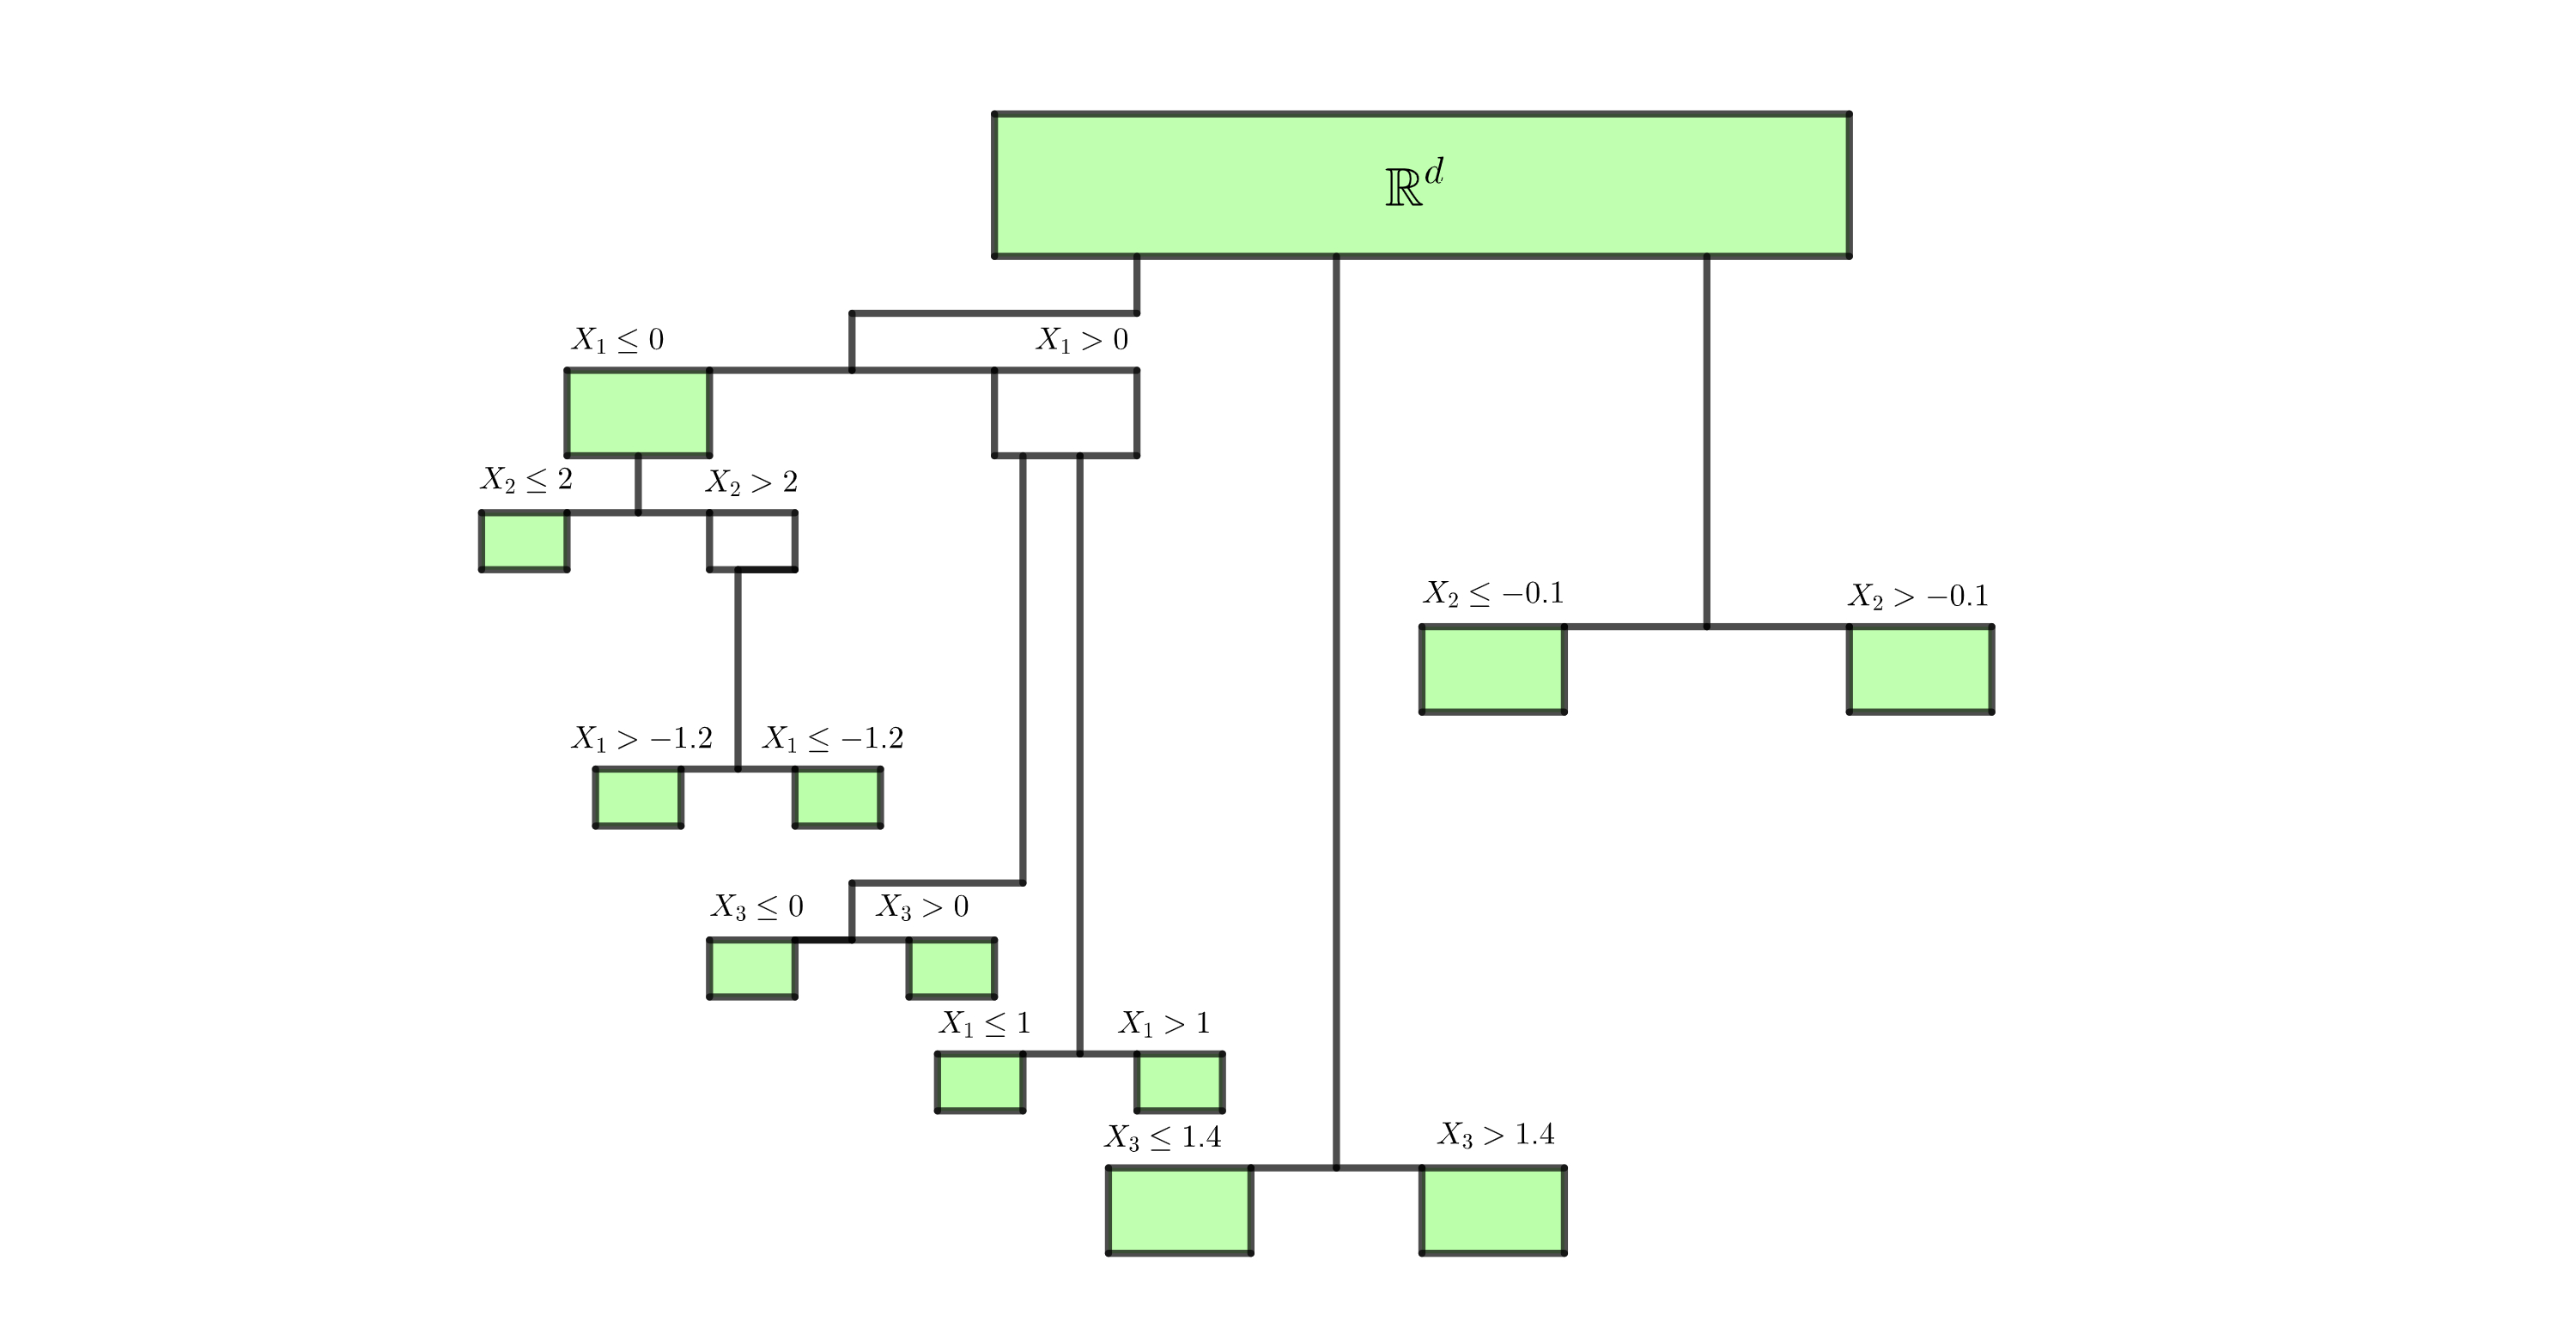
\includegraphics[width=1.2\linewidth]{img/2023_paper_skizze_Planted_Tree.jpg}
        \vspace{-10pt}
        % \caption{Structure of Ewald Message Passing}
        \label{fig:Figure_Ewald-MP_Algo_Structure}
    \end{figure}
    
\end{frame}



\subsection{Related work and new contributions}

\begin{frame}{Related work and new contributions}
    
    \textbf{Other low-order methods:}
    \begin{itemize}
        \item GAMs, e.g. tree-based explainable boosting machine\\
        (Lengerich, Tan, Chang, Hooker, and Caruana (2020))
        \item neural network based neural additive model\\
        (Agarwal, Frosst, Zhang, Caruana, and Hinton (2020))
    \end{itemize}

    \textbf{Comparisons for theoretical results:}
    \begin{itemize}
        \item Random forests
        \item[\(\rightarrow\)] RFs with trees growing in parallel (Tan, Agarwal, and Yu (2022))
        \item[\(\leftrightarrow\)] theoretical analysis here following Biau, Devroye, and Lugosi (2008) and Biau (2012)
    \end{itemize}

    \textbf{Further methods to compare to:}
    \begin{itemize}
        \item MARS (Friedman (1991))
        \item XGBoost
        \item BART
    \end{itemize}
    
\vspace{1cm}

\end{frame}



\section{The RPF method in detail}





\subsection{Building Forests}

\begin{frame}{General algorithm: Building Random Forests}

    \begin{itemize}
        \item \texttt{n\textunderscore trees} many trees 
        \item \texttt{n\textunderscore splits} many splits per tree
        \item forest estimator \(=\) average over single tree estimators\\
        bootstrap sampling
        \item Given maximum interaction order \texttt{max\textunderscore interaction} or \(r\)
        \item For each split: Choose leaf, splitting coordinate \& splitting value
    \end{itemize}
    
\vspace{1cm}

\end{frame}



\subsection{Splitting Leaves}

\begin{frame}{Splitting Leaves and Calculating Estimator}

    Assume a leaf, a splitting coordinate, and a splitting value has been chosen

    \vspace*{.5cm}

    \textbf{$\rightarrow$ Delete this leaf or not?}

    \hspace*{.5cm} $\rightarrow$ Here: Delete \(\Leftrightarrow\) Splitting variable has occurred before

    \vspace*{.5cm}

    \textbf{$\rightarrow$ How to calculate estimator value for new leaves?}

    \begin{center}
    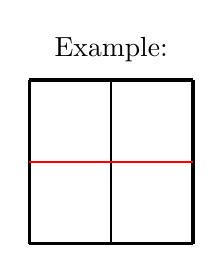
\begin{tikzpicture}[
    node/.style = {draw, circle, scale=0.4},
    scale = .13
    ]   

        \node[] at (8,19)(Level_0){Example:};
        
        \foreach \shift in {0}{
            \draw[very thick]{} (\shift,0) -- (\shift +16,0);
            \draw[very thick]{} (\shift +16,0) -- (\shift +16,16);
            \draw[very thick]{} (\shift +0,0) -- (\shift +0,16);
            \draw[very thick]{} (\shift +0,16) -- (\shift +16,16);
        }

        \foreach \shift in {0}{
            \draw[thick]{} (\shift +8,0) -- (\shift +8,16);
            \draw[thick, red]{} (\shift +0,8) -- (\shift +16,8);
        }
        
    \end{tikzpicture}
    \end{center}

    \hspace*{.5cm} $\rightarrow$ Use average residual
    
    $\Rightarrow$ Order in which splits occur influences final estimator
    


\end{frame}

\begin{frame}{Splitting Leaves and Calculating Estimator}

    \begin{figure}[h]
        \centering
        \vspace{-10pt} % Note that this is only to ensure a normal, not to big margin around the figure
        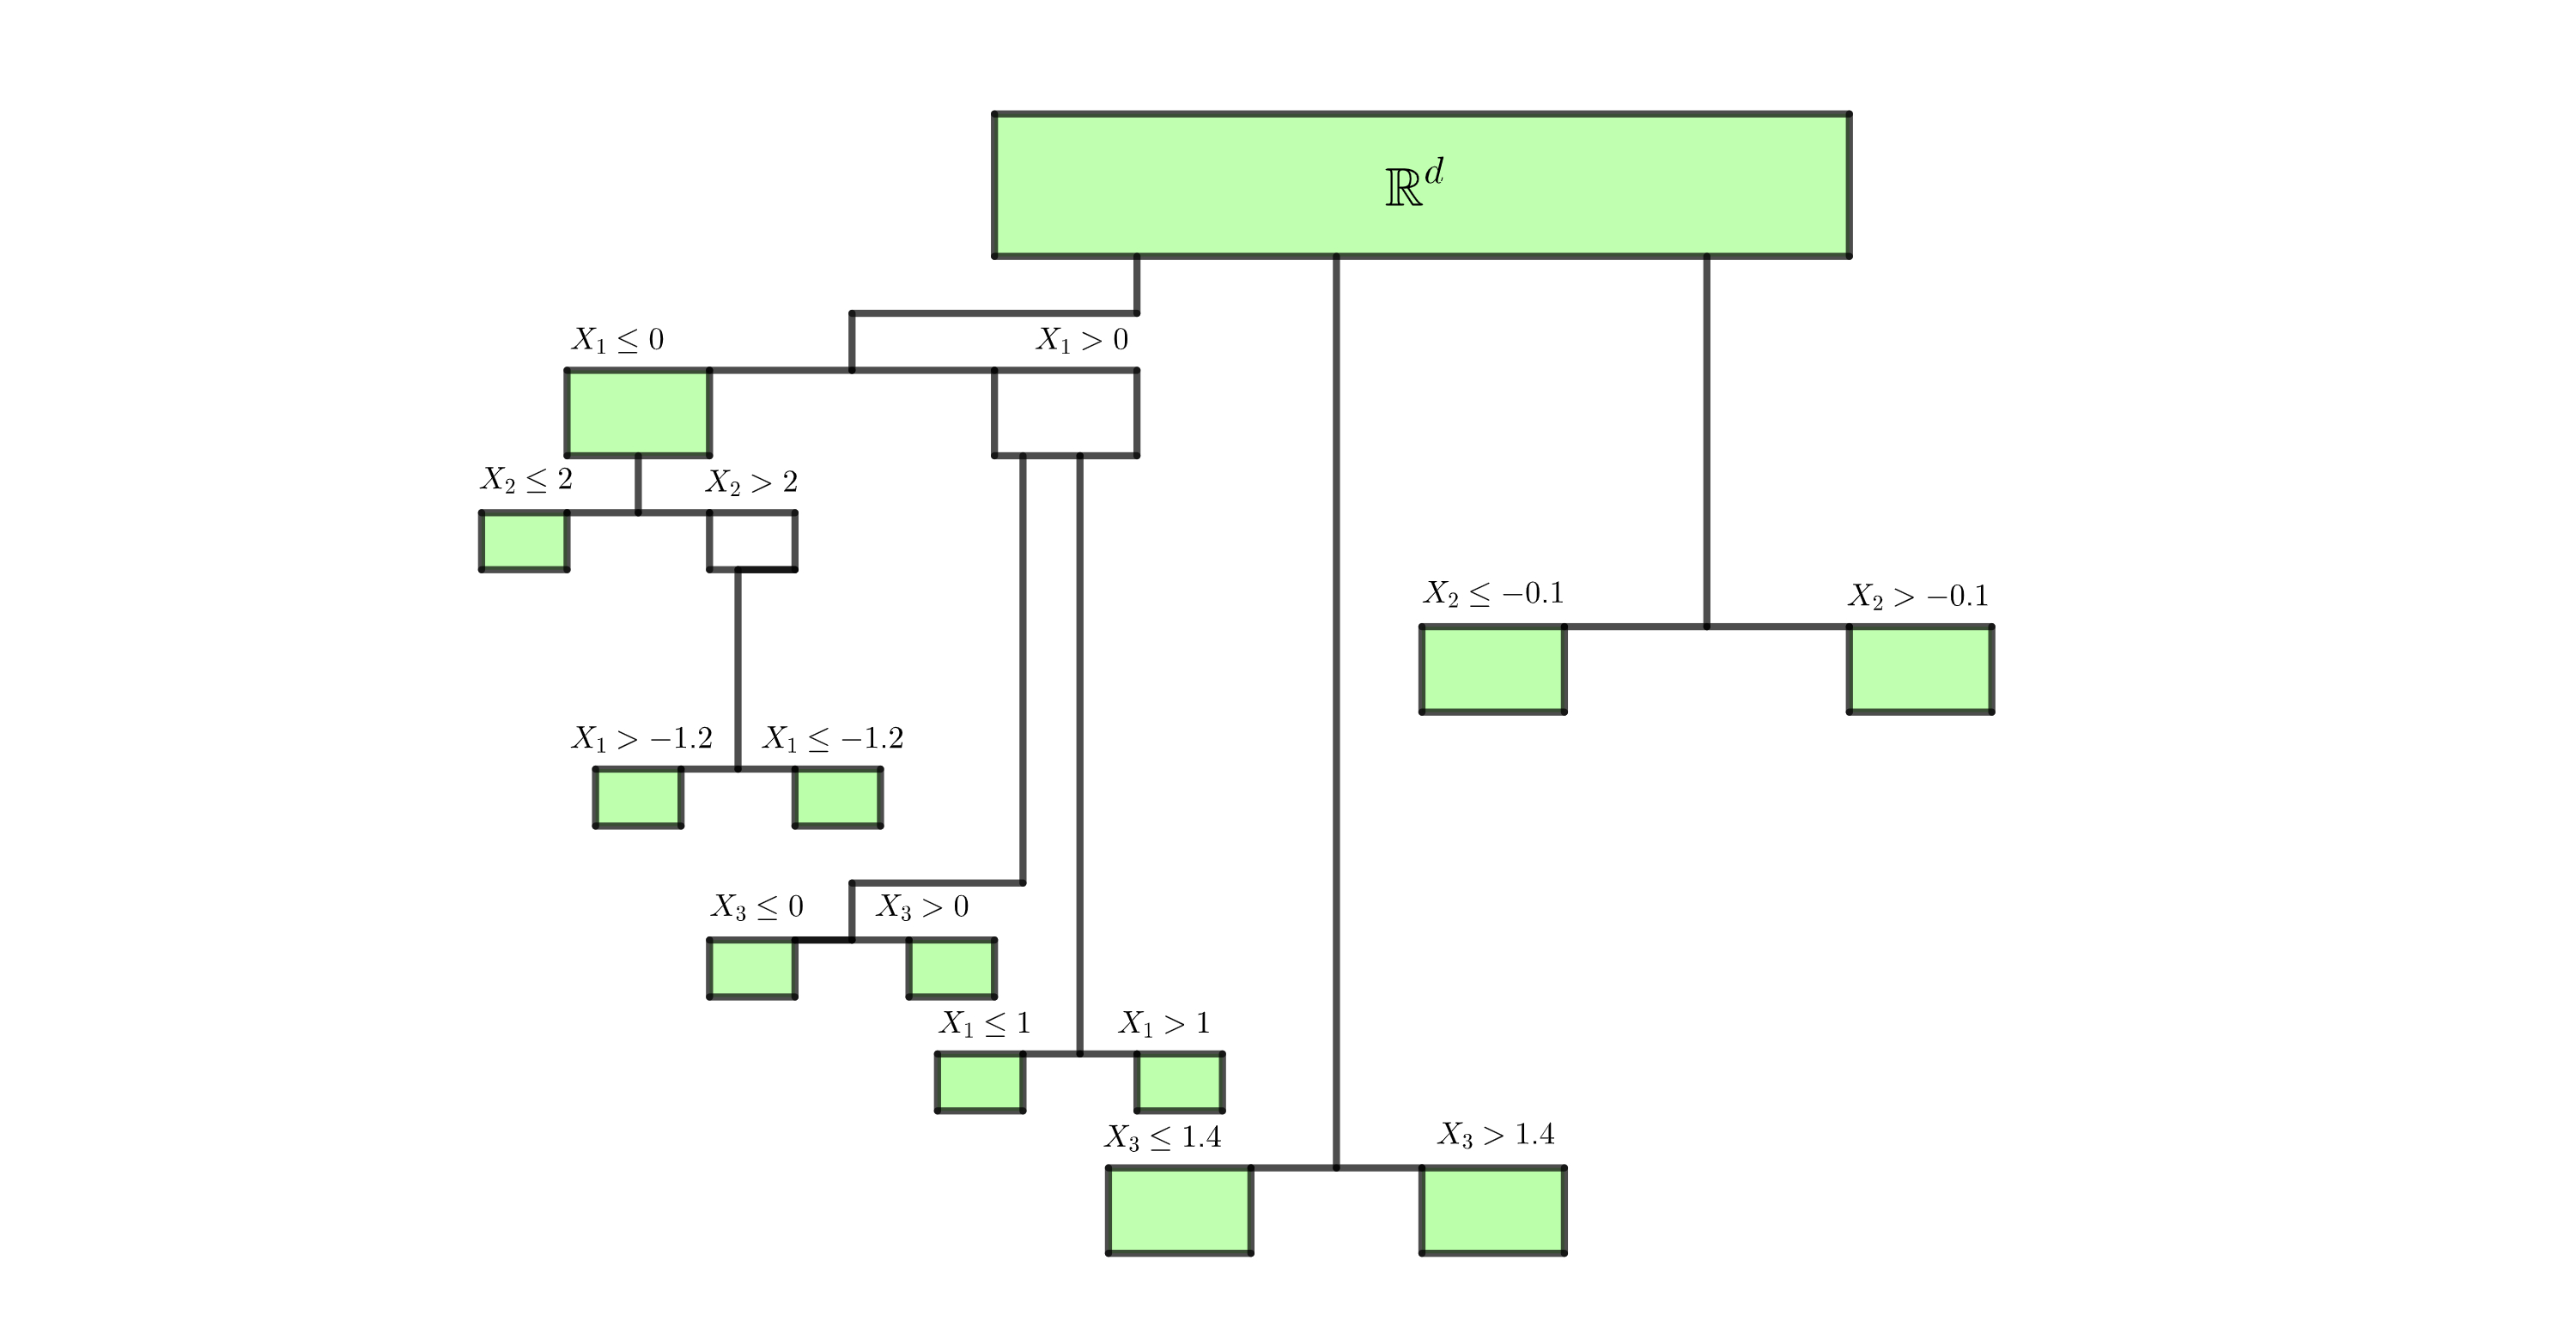
\includegraphics[width=1.2\linewidth]{img/2023_paper_skizze_Planted_Tree.jpg}
        \vspace{-10pt}
        % \caption{Structure of Ewald Message Passing}
        \label{fig:Figure_Ewald-MP_Algo_Structure}
    \end{figure}
    
\end{frame}

%TODO: formula for algo

%\begin{frame}{Splitting Leaves and Calculating Estimator}

%    TODO formula

%\end{frame}



\subsection{Choosing Splits}



\begin{frame}{Choosing Splits: \(\approx\) CART method}

    Brute-force minimize the total residual after the split

    BUT: Only certain (leaf type)-(splitting coordinate) combinations \((t, k)\) are allowed: \( \left| t \cup \{k\} \right| \leq r \)

    \vspace*{.5cm}

    \textbf{From random forests: Variant of feature bagging}

    \hspace*{.5cm} $\rightarrow$ Of all possible combinations, uniformly at random choose a subset of proportion \texttt{t\textunderscore try} to optimize over

    \hspace*{.5cm} $\rightarrow$ Of all possible split values, uniformly at random choose \texttt{split\textunderscore try} many of them to optimize over

\end{frame}



\section{Experimental results}



\subsection{Setup}

\begin{frame}{Setup of Experiments: Problems}

    \begin{figure}[h]
        \centering
        \vspace{-10pt} % Note that this is only to ensure a normal, not to big margin around the figure
        \includegraphics[width=\linewidth]{img/Bildschirmfoto_20241015_010319_table_overview_problems.png}
        \vspace{-10pt}
        % \caption{Structure of Ewald Message Passing}
        \label{fig:Figure_Ewald-MP_Algo_Structure}
    \end{figure}
    
\end{frame}



\subsection{Results}

\begin{frame}{Experimental Results}

    \begin{figure}[h]
        \centering
        \vspace{-10pt} % Note that this is only to ensure a normal, not to big margin around the figure
        \includegraphics[width=1.05\linewidth]{img/Bildschirmfoto_20241015_010402_results_table_03.png}
        \vspace{-10pt}
        % \caption{Structure of Ewald Message Passing}
        \label{fig:Figure_Ewald-MP_Algo_Structure}
    \end{figure}
    
\end{frame}

\begin{frame}{Experimental Results}

    \begin{figure}[h]
        \centering
        \vspace{-10pt} % Note that this is only to ensure a normal, not to big margin around the figure
        \includegraphics[width=\linewidth]{img/Bildschirmfoto_20241015_111636_results_table_07.png}
        \vspace{-10pt}
        % \caption{Structure of Ewald Message Passing}
        \label{fig:Figure_Ewald-MP_Algo_Structure}
    \end{figure}
    
\end{frame}

\begin{frame}{Experimental Results}

    \begin{figure}[h]
        \centering
        \vspace{-10pt} % Note that this is only to ensure a normal, not to big margin around the figure
        \includegraphics[width=\linewidth]{img/Bildschirmfoto_20241015_111755_results_table_09.png}
        \vspace{-10pt}
        % \caption{Structure of Ewald Message Passing}
        \label{fig:Figure_Ewald-MP_Algo_Structure}
    \end{figure}
    
\end{frame}

\begin{frame}{Experimental Results}

    \begin{figure}[h]
        \centering
        \vspace{-10pt} % Note that this is only to ensure a normal, not to big margin around the figure
        \includegraphics[width=\linewidth]{img/Bildschirmfoto_20241015_111844_results_table_13.png}
        \vspace{-10pt}
        % \caption{Structure of Ewald Message Passing}
        \label{fig:Figure_Ewald-MP_Algo_Structure}
    \end{figure}
    
\end{frame}



\subsection{Discussion}

\begin{frame}{Discussion of Experimental Results}
    
    \begin{itemize}
        \item High flexibility of RPFs w.r.t. interaction order
        \item RPF are better in detecting interactions in sparse problems?
        \item RPFs not so good for smooth problems? Better for non-regular problems?
        \item RPFs complementary to other popular methods (XGBoost, standard RFs)
    \end{itemize}
    
\vspace{1cm}

\end{frame}



\section{Theoretical results}



\begin{frame}{Theoretical results: Setup}
    
    \textbf{Slightly different algorithm:}
    \begin{itemize}
        \item Different definition of leaf type
        \item One planted tree is now an ensemble (i.e. sum) of classical decision trees, one for each leaf type
        \item Splits are chosen randomly, not by minimization \(\Rightarrow\) neglects CART
        \item After each split, update not only the estimator values for the 2 new leaves, but for all leaves in the current sub-tree
        \item Neglecting bootstrap samples
    \end{itemize}

    Then rewrite the update rule of the estimator values in new leaves as an integral using the density estimator.

\end{frame}

\begin{frame}{Theoretical results: Assumptions}

    Important tool in the proof: Density estimators (Histogram estimators) and their convergence
    
    \textbf{Assumptions:}
    \begin{itemize}
        \item target function is in \(\mathcal{C}^2\)
        \item data points and errors are i.i.d., centered, densities are in \(\mathcal{C}^2\)
        \item single DT-groups are i.i.d.
        \item Towards the end (\(\approx\) last \(\log^2(n)\) splits), each leaf type is chosen often enough
        \item Tree partitions become fine enough, side length of leaves (\grqq bandwidth\grqq \(h\)) goes to zero slow enough
        \item Changes in the last \(\approx \log^2(n)\) splits are not too large, both regarding the side length of new leaves as well as changes to the estimator
        \item histogram estimators (for each tree) converge to the underlying distribution, as well as histogram estimators of joint density (in multiple senses)
        \item average histogram estimator (over all trees) converges to underlying distribution
    \end{itemize}

    %\textbf{Assumptions for all the single planted trees:}
    %\begin{itemize}
    %    \item target function is in \(\mathcal{C}^2\)
    %    \item data points and errors are i.i.d., centered, densities are in \(\mathcal{C}^2\)
    %    \item single DT-groups are i.i.d.
    %    \item Towards the end (\(\approx\) last \(\log^2(n)\) splits), each leaf type is chosen often enough
    %    \item Tree partitions become fine enough, side length of leaves (\grqq bandwidth\grqq \(h\)) goes to zero slow enough
    %    \item Changes in the last \(\approx \log^2(n)\) splits are not too large, both regarding the side length of new leaves as well as changes to the estimator
    %    \item histogram estimators (for each tree) converge to the underlying distribution, as well as histogram estimators of joint density (in multiple senses)
    %    \item average histogram estimator (over all trees) converges to underlying distribution
    %\end{itemize}
    
\vspace{1cm}

\end{frame}

\begin{frame}{Theoretical results: Results}

    \textbf{Results:}
    \begin{itemize}
        \item For trees:

        \begin{center}
            Convergence of every single planted tree estimator in \(L^2\) with convergence rate:
            \(\OOO \left( \left( \log(n) \right)^{-2} + \sqrt{\frac{S}{n}} \right) \)
        \end{center}
        
        \item For forests:

        \begin{center}
            Convergence of total forest estimator in \(L^1\) with convergence rate:\\
            \( \left( \log(n) \right)^{-2} + \sqrt{\frac{S}{n}} + \delta_{3,n}^2 + \delta_{4,n}\) \\
            \(\leq h^2 + h(nh^{2r})^{-1/2} + (nh^{r})^{-1/2}\)
        \end{center}
        
        \item In particular for cases \(r=1\) and \(r=2\): Forests achieve optimal convergence rate

        \begin{center}
        for \(r=1\): rate \(n^{-2/5}\); for \(r=2\): rate \(n^{-1/3}\)
            
        \end{center}
        
    \end{itemize}
    
\vspace{1cm}

\end{frame}



\section{Outlook and Open Questions}



% \subsection{Summary ???}

\begin{frame}{Outlook and Open Questions}
    
    \textbf{Concerning the implementation and the experiments:}
    \begin{itemize}
        \item How exactly was the hyperparameter search done? Grid search?
        \item experiments on real-world datasets, concerning both performance and interpretability
        \item experiments on problems of order 3 or higher
        \item better explanation or intuition for why to keep or delete certain nodes
    \end{itemize}

    \textbf{Concerning the theory:}
    \begin{itemize}
        \item theory for data-dependent splitting (e.g. CART) \& for sub-sampling
        \item Is this the first theoretical result proving optimal convergence rates for decision tree ensembles?
    \end{itemize}

    Are planted trees also useful for standard random forests?
    
\vspace{1cm}

\end{frame}




\end{document}
